\begin{frame}
  \frametitle{Reciprocal Inconsistency}
  Distributed edge $ab$ indicates \texttt{Tolkien} wrote \texttt{The Hobbit}
  \begin{figure}
    \centering
    \input{./figures/dist-edge}
    \caption{Distributed edge}
  \end{figure}
\end{frame}

\begin{frame}
  \frametitle{Reciprocal Inconsistency}
  \begin{itemize}
  \item $T_x$ deletes the edge
  \item $T_y$ appends a property \textcolor{red}{\texttt{year}}
  \end{itemize}

  \begin{figure}
    \centering
    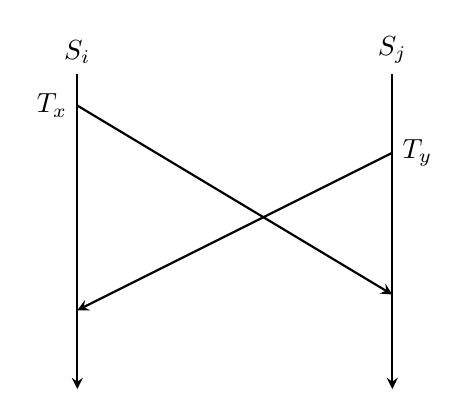
\begin{tikzpicture}
      \draw [thick,<-,>=stealth] (0,0) -- (0,4) node[anchor=south] {$S_i$};
      \draw [thick,<-,>=stealth] (4,0) -- (4,4) node[anchor=south] {$S_j$};
      \draw [thick,<-,>=stealth] (0,1) -- (4,3)  node[right] {$T_y$};
      \draw [thick,->,>=stealth] (0,3.6) node[left] {$T_x$} -- (4,1.2);
    \end{tikzpicture}
  \end{figure}
\end{frame}

\begin{frame}
  \frametitle{Reciprocal Inconsistency}
  The distributed edge is now reciprocally inconsistent
  \begin{figure}
    \centering
    \begin{tikzpicture}[node distance=2.2cm]
    \node (rect)  [draw,rounded corners,minimum width=3.5cm,minimum height=4cm,label=above:{$S_i$}] {};
  \node (rect)  [draw,rounded corners,minimum width=3.5cm,minimum height=4cm,label=above:{$S_j$},xshift=5.6cm] {};
  \node (v1) [big_vertex,xshift=0cm,yshift=0cm] {\small{\texttt{a:\textcolor{green}{Person}}}};

  \node (v2) [big_vertex,xshift=5.6cm,yshift=0cm] {\small{\texttt{b:\textcolor{green}{Book}}}};

  \node [below of=v1,yshift=1cm] {\small{\texttt{\textcolor{red}{name}:Tolkien}}};
  \node [below of=v2,yshift=1cm] {\small{\texttt{\textcolor{red}{title}:The Hobbit}}};

  \draw [thick,dashed,->,>=stealth] (0.9,0)  -- node [midway,above] {:\textcolor{green}{\small{\texttt{WROTE}}}} node [midway,below,xshift=0.1cm] {\small{\texttt{\textcolor{red}{year}:1937}}} (2.7,0);
\end{tikzpicture}

    \caption{Reciprocally inconsistent distributed edge}
  \end{figure}
\end{frame}

\begin{frame}
  \frametitle{Reciprocal Inconsistency}
Storage representation consists of two inconsistent unidirectional edges

\begin{figure}
\centering
\begin{subfigure}{.5\textwidth}
  \centering
  \includegraphics[width=.9\linewidth]{./images/si}
  \caption{$S_i$}
  \label{fig:sub1}
\end{subfigure}%
\begin{subfigure}{.5\textwidth}
  \centering
  \includegraphics[width=.9\linewidth]{./images/sj}
  \caption{$S_j$}
  \label{fig:sub2}
\end{subfigure}
\caption{Storage representation}
\label{fig:test}
\end{figure}
\end{frame}

\begin{frame}
  \frametitle{Reciprocal Inconsistency}
  \begin{itemize}
  \item Reciprocally inconsistent edges are the source for \emph{semantic corruption}
  \item Semantic corruption spreads until the database becomes \emph{operationally corrupt}
  \item \textbf{Motivated the design of a lightweight protocol that preserves reciprocal consistency}
  \end{itemize}
\end{frame}